\providecommand{\pdfxopts}{a-1b,cyrxmp}
\providecommand{\thisyear}{2020}
\immediate\write18{rm \jobname.xmpdata}%  uncomment for Unix-based systems
\begin{filecontents*}{\jobname.xmpdata}
\Title{Силовая электроника. Виртуальная лабораторная работа №2\textemdash\thisyear}
\Author{Артем Николаевич Прокшин}
\Creator{pdfTeX + pdfx.sty with options \pdfxopts }
\Subject{Виртуальная лабораторная работа №2
\sep
исследование неуправляемых
\sep
выпрямителей и фильтров
\sep
выпрямленного тока}
\Keywords{неуправляемый выпрямитель, фильтры, ЛЭТИ}
\CoverDisplayDate{апрель \thisyear}
\CoverDate{2020-04-04}
\Copyrighted{True}
\Copyright{Public Domain}
\CopyrightURL{http://github.com/trot-t}
\Creator{pdfTeX + pdfx.sty with options \pdfxopts }
\end{filecontents*}

\documentclass[a4paper,12pt]{article}

\pdfcompresslevel=9

\usepackage[\pdfxopts]{pdfx}[2016/04/04]
\PassOptionsToPackage{obeyspaces}{url}
\let\tldocrussian=1  % for live4ht.cfg


\usepackage{extsizes} 
\usepackage[left=10mm, top=20mm, right=10mm, bottom=20mm, nohead, footskip=7mm]{geometry} % настройки полей документа


\usepackage[T2A]{fontenc}
\usepackage[utf8]{inputenc}
\usepackage[english,russian]{babel}
\usepackage{tikz}
\usetikzlibrary{positioning}
\usepackage[european,cuteinductors,smartlabels,siunitx]{circuitikz}

%% 
\usepackage{pdflscape}
\usepackage{afterpage}

%%% Межстрочный интервал
\usepackage{setspace}

%% таблицы
\usepackage{booktabs}
%multi-row
\usepackage{multirow}

%% для кода
\usepackage{color}
\usepackage{listingsutf8}

%\input{colors}
\definecolor{lightgrey}{rgb}{0.9,0.9,0.9}
\definecolor{lightblue}{rgb}{0,0,1}

\definecolor{grey}{rgb}{0.5,0.5,0.5}
\definecolor{blue}{rgb}{0,0,1}
\definecolor{violet}{rgb}{0.5,0,0.5}

\definecolor{darkred}{rgb}{0.5,0,0}
\definecolor{darkblue}{rgb}{0,0,0.5}
\definecolor{darkgreen}{rgb}{0,0.5,0}


\lstset{%
  language=C++,%
  morekeywords={constexpr,nullptr,size_t,uint32_t,assert,override,final},%
  basicstyle=\ttfamily\footnotesize,%
  sensitive=true,%
  keywordstyle=\color{blue},%
  stringstyle=\color{darkgreen},%
  commentstyle=\color{violet},%
  showstringspaces=false,%
  tabsize=2,%
  frame=leftline,
  rulecolor=\color{lightblue},
  xleftmargin=20pt,
}

\lstset{
%extendedchars=\true,
%inputencoding=utf8x,   
  numberstyle=\tiny,
  numbers=left,
  numbersep=10pt,
  xleftmargin=20pt,
  %framesep=4.5mm,
  %framexleftmargin=2.5mm,
  framexleftmargin=5pt,
  framesep=15pt,
  fillcolor=\color{lightgrey},
}


\title{Исследование неуправляемых выпрямителей и фильтров выпрямленного тока}
\author{Artem N Prokshin}
% Конец преамбулы
\begin{document}
%\maketitle
%\begin{tikzpicture}
%\newcommand{\xb}{-3}
%\newcommand{\xa}{3}
%\draw[thin, ->] (-6,0) -- (6,0) node[right] {$X$};
%\draw[thin, ->] (0,-6) -- (0,6) node[left] {$Y$};
%\foreach \x\xtext in {-5/-5,5/5,{\xb}/\xb,{\xa}/{\displaystyle \frac{-b+\sqrt{b^2-4ac}}{2a}}} % 
%   \draw (\x,0.1) -- (\x,-0.1) node[below] {$\xtext$};

 %\draw[domain=-5:5, help lines, smooth]
 %       plot ({\x},{0.2*(\x-\xa)*(\x-\xb)});
%\end{tikzpicture}

\section{Исследование неуправляемых выпрямителей и фильтров выпрямленного тока}

{\bf Целью} работы является исследование характеристик различных вариантов схем неуправляемых выпрямителей однофазного напряжения 
и влияние на их работу сглаживающих фильтров.
 
\subsection{Виртуальная установка для исследования свойств неуправляемых выпрямителей} 

\begin{figure}[!ht]
\centering
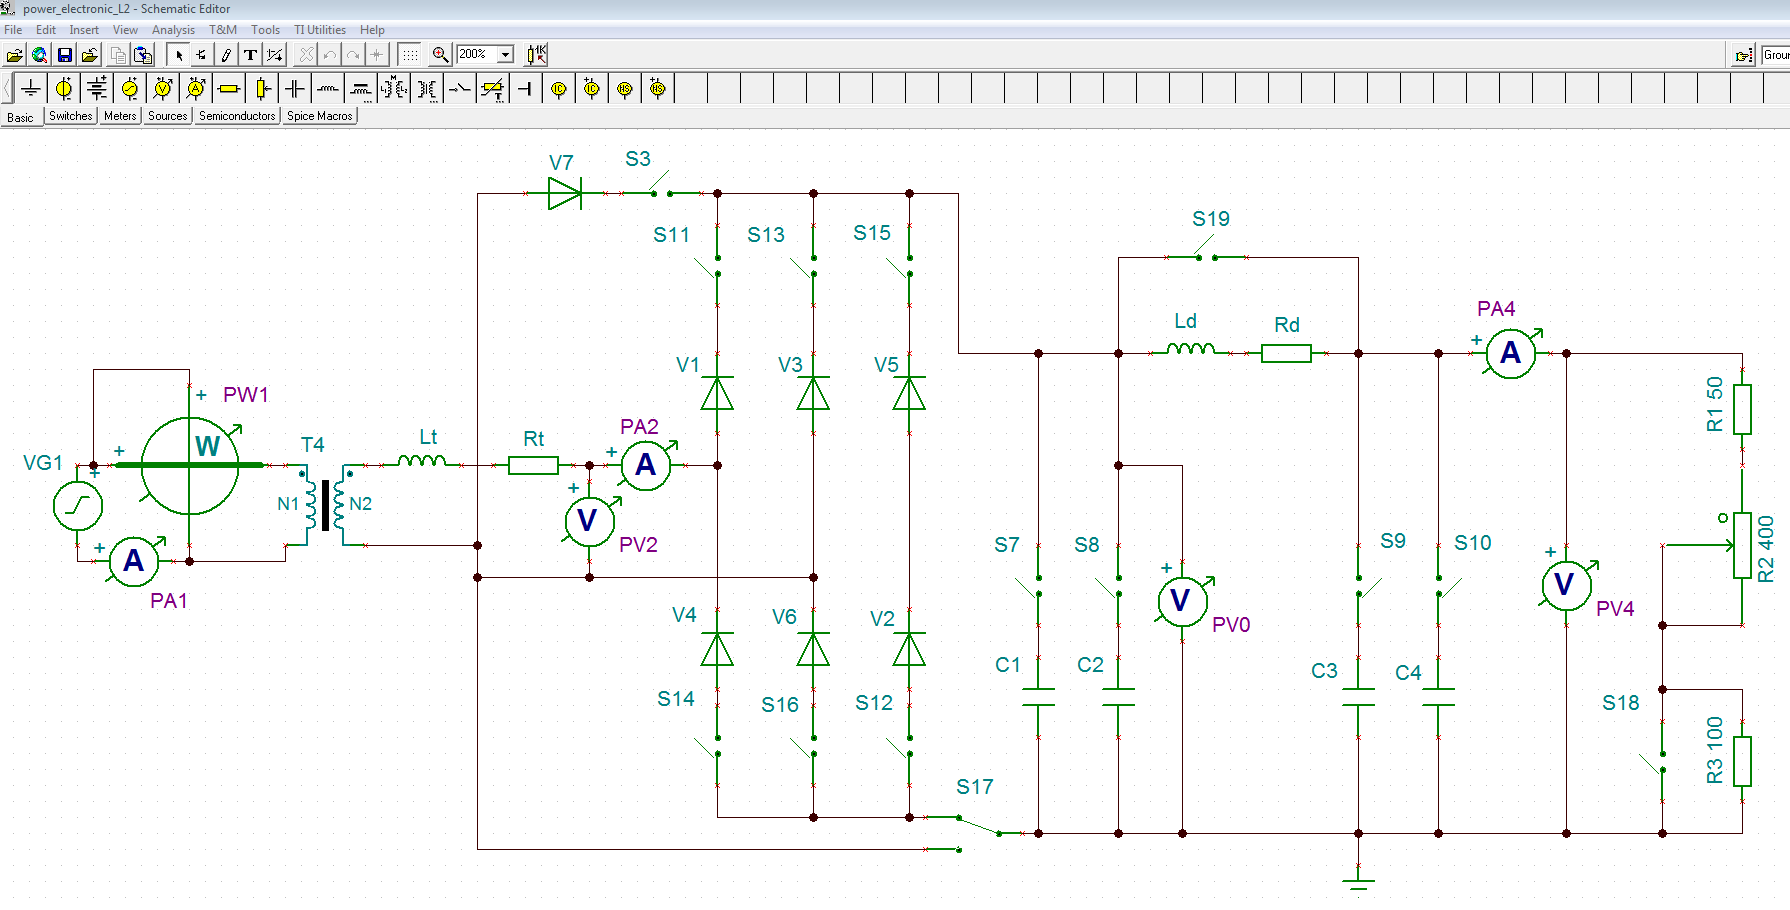
\includegraphics[scale=0.4, angle=90]{setup_lab2}
\caption{схема виртуальной установки для исследования свойств неуправляемых выпрямителей}
\label{setup}
\end{figure}

Виртуальная установка, представленная на схеме \ref{setup}, запускается с помощью программы \href{http://www.ti.com/tool/TINA-TI}{tina} с бесплатной лицензией.

На виртуальной установке с помощью тумблеров можно исследовать следующие схемы выпрямителей:

\begin{enumerate}
\item \label{one-phase-half-period} однофазную однополупериодную;
\item \label{one-phase-half-period-with-shunt} однофазную однополупериодную с шунтирующим диодом;
\item \label{two-half-period} однофазную двухполупериодную с выведенной нулевой точкой на вторичной обмотке преобразовательного трансформатора;
\item \label{one-phase-bridge} однофазную мостовую.
\end{enumerate}

Далее следовать методике описанной в \href{https://github.com/trot-t/power_el_method_old/blob/master/%D0%A1%D0%B8%D0%BB%D0%BE%D0%B2%D0%B0%D1%8F%20%D1%8D%D0%BB%D0%B5%D0%BA%D1%82%D1%80%D0%BE%D0%BD%D0%B8%D0%BA%D0%B0%20%D0%BC%D0%B5%D1%82%D0%BE%D0%B4%D0%B8%D1%87%D0%BA%D0%B0%20%D0%BB%D0%B0%D0%B1%D0%BE%D1%80%D0%B0%D1%82%D0%BE%D1%80%D0%BD%D1%8B%D0%B5.pdf}{методичке} для реальной лабораторной установке.


\subsection{порядок выполнения измерений на виртуальной установке}

\begin{itemize}
	\item Открыть \href{https://github.com/trot-t/power_electronics_virtual_labs/blob/master/power_electronic_L2.TSC}{схему 
		для пунктов} \ref{one-phase-half-period}, \ref{one-phase-half-period-with-shunt}, \ref{one-phase-bridge} 
		или \href{https://github.com/trot-t/power_electronics_virtual_labs/blob/master/power_electronics_L2_tap.TSC}{схему 
		для пункта \ref{two-half-period}}
		в программе \href{http://www.ti.com/tool/TINA-TI}{tina};
\item С помощью тумблеров $S_3,S_{11},S_{13},S_{14},S_{16}, S_{17}$ составить схему выпрямителя, указанную преподавателем;
\item Выбрать в меню анализ $\Rightarrow$ переходных процессов (transient analisys) $\Rightarrow$ для нескольких периодов колебаний 
	входной сети, 
	например, с момента времени 40 мс до 100 мс.
\begin{figure}[!ht]
\centering
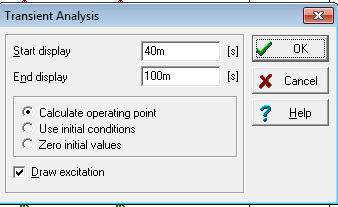
\includegraphics[scale=0.4]{analisys}
\caption{выбор начального и конченого времен в анализе переходных процессов}
\label{analisys}
\end{figure}	

\item получаем графики для мгновенных значений токов и напряжений: 
\begin{figure}[!ht]
\centering
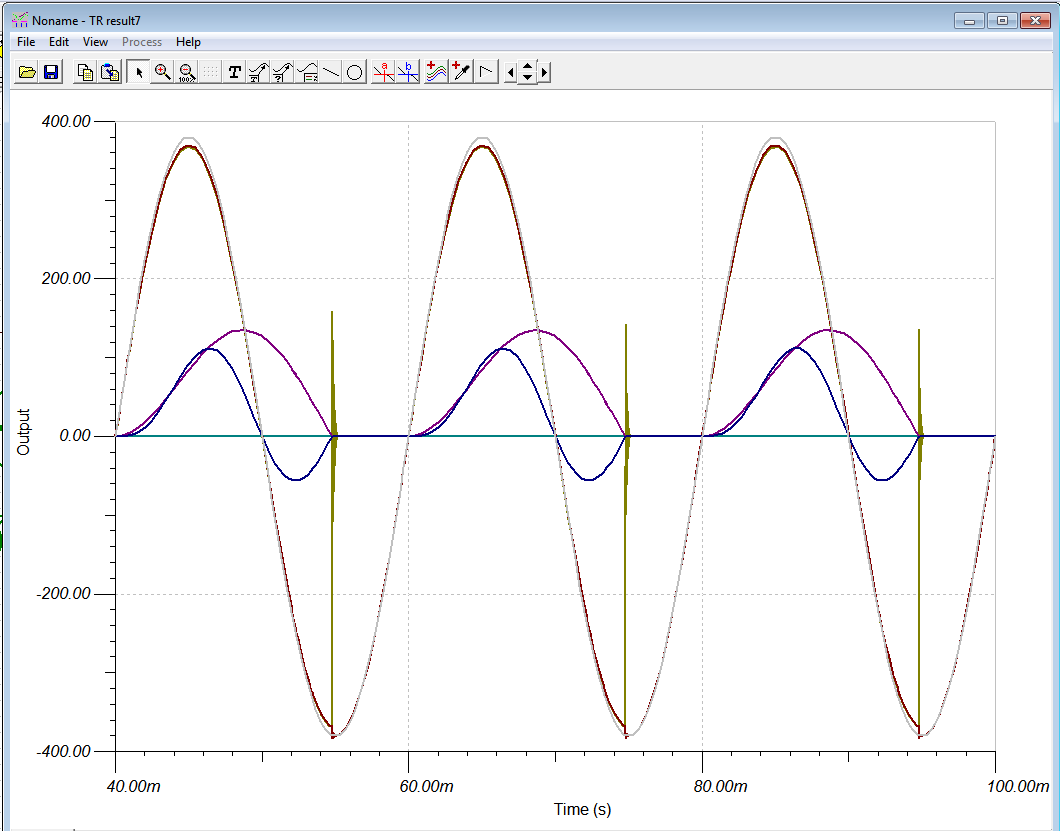
\includegraphics[scale=0.3]{result}
\caption{результат анализа переходных процессов}
\label{result}
\end{figure}	

\item Можно отобразить отдельную кривую <<show/hide curves>>. Также можно разобрать кривые по отдельным графикам. 
	Для этого в меню графика выбрать <<split curves>>
\begin{figure}[!ht]
\centering
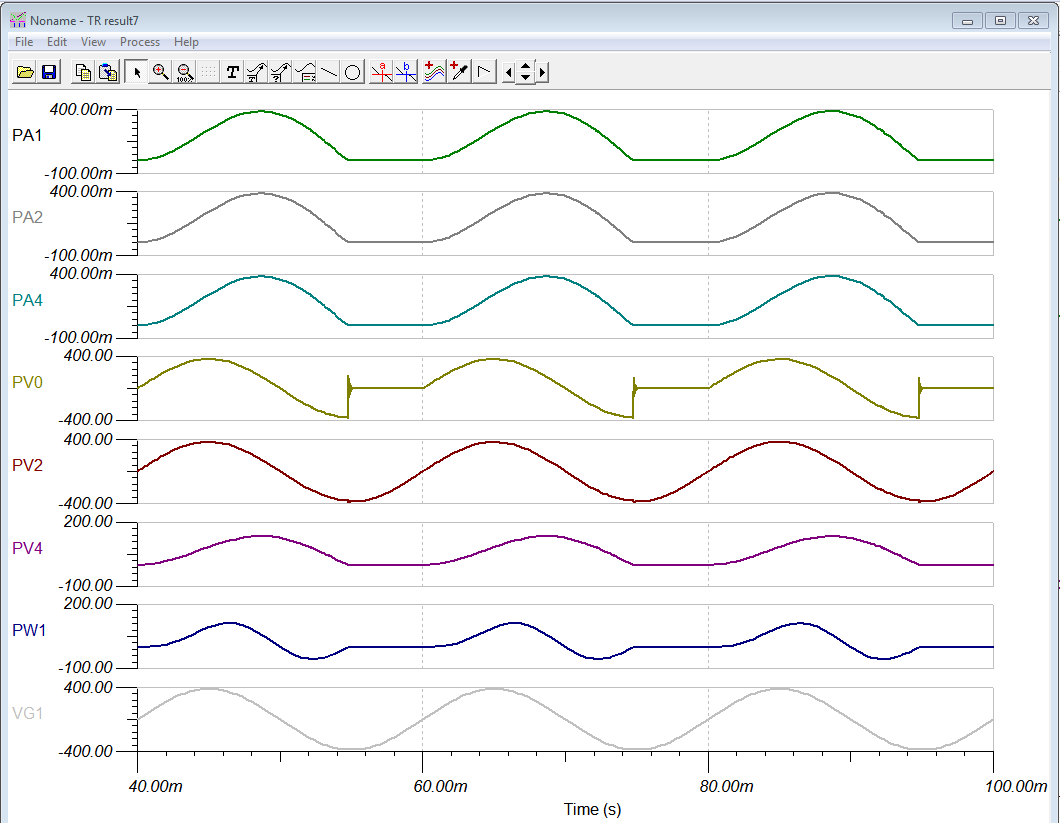
\includegraphics[scale=0.3]{result_splitted}
\caption{отдельные графики токов и напряжений}
\label{result_splitted}
\end{figure}  

\item В реальной установке для измерения действующих значений и средних значений используются приборы с различной
	измерительной системой. В виртуальной установке для получения действующих значений и средних значений
	выбрать график параметра, например, $PV4$ мышью, в меню графика выбрать Process $\Rightarrow$ <<Averages...>>.
\begin{figure}[!ht]
\centering
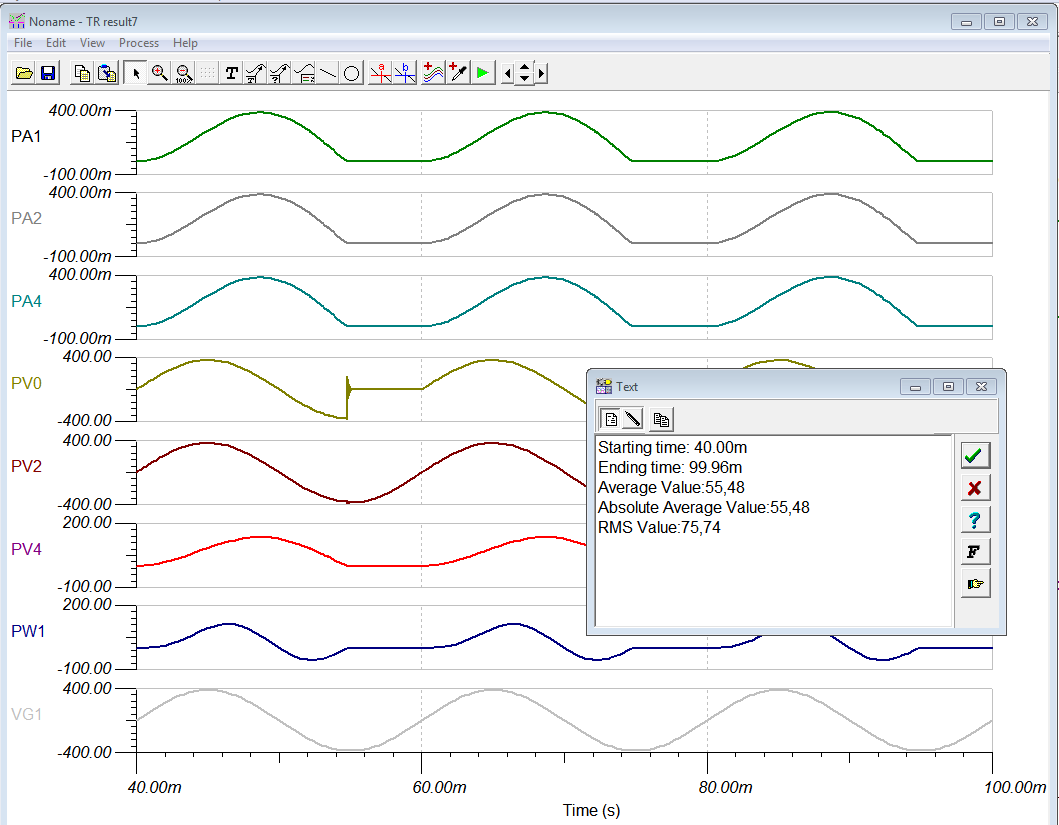
\includegraphics[scale=0.3]{result_rms_avg}
\caption{действующие и средние значения}
\label{result_rms_avg}
\end{figure}

\item параметры дросселя изменять в соответствии с параметрами реальной установки:
\begin{table}[!ht]
\centering
\begin{tabular}{l|l|l}
\toprule
	2-е положение& $L_d$=0,394 Гн& $R_d$= 11 ом \\
\midrule
        3-е положение& $L_d$=0,86 Гн& $R_d$= 19,3 ом \\
\midrule
        4-е положение& $L_d$=2,12 Гн& $R_d$= 29,3 ом \\
\midrule
        5-е положение& $L_d$=4,07 Гн& $R_d$ = 38 ом \\
\bottomrule
\end{tabular}
	\caption{параметры дросселя}
\end{table}

\item прочие параметры также соответствуют параметрам реальной установки:
\begin{table}[!ht]
\centering
\begin{tabular}{lcl}
\toprule
	$R_\textcyrillic{трансформатора}$ &=& 8 ом\\
%\midrule
	$R_\textcyrillic{вентиля динамическое}$ &=& 1,6 ом\\
%\midrule
	$x_a$ &=& 37 ом \\
%\midrule
	$U_\textcyrillic{о.вентиля}$ &=& 0,4 В \\
\bottomrule
\end{tabular}
\caption{Прочие параметры}
\end{table} 
\end{itemize}

%\subsection{фотография реальной установки}
\begin{figure}[!ht]
\centering
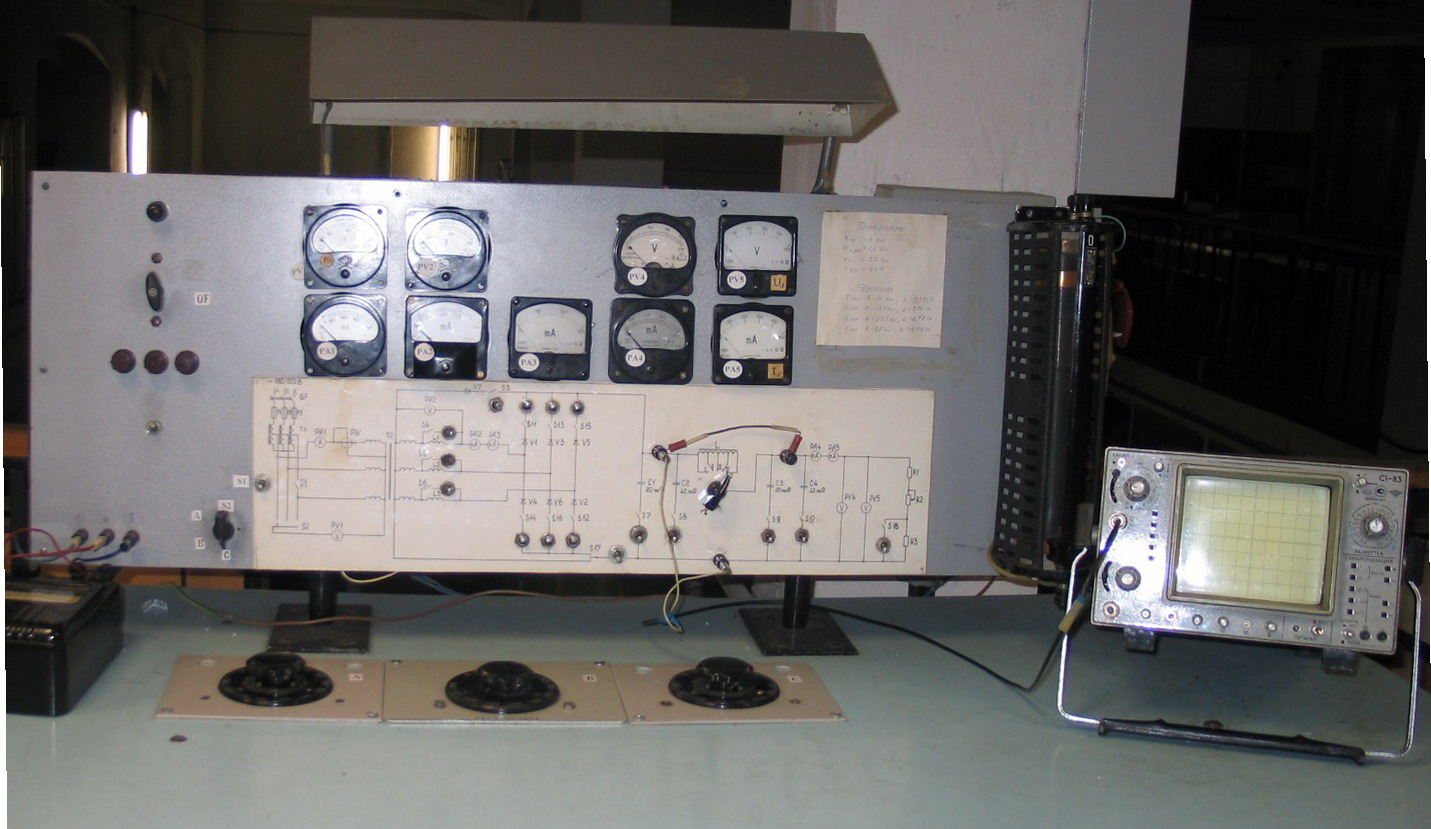
\includegraphics[scale=0.8]{lab2_real}
\caption{фотография реальной лабораторной установки}
\label{result_rms_avg}
\end{figure}



\afterpage{%
\newgeometry{left=20mm, top=0mm, right=20mm, bottom=2mm, nohead}
% material for this page
\begin{landscape} 
	\hspace{-0.2cm}
\begin{figure}[!ht]
\begin{circuitikz}[scale=0.85, yscale=1.1]
  \draw[color=black, thin]
  (1,0) node[above right] {380В}
(-0.1,-1)--(2.9,-1)
(-0.2,-0.8)--(2.8,-0.8)
%(0,-1) to [short, -o] (0,0)
(0,-2) to [nos,-o] (0,0)
%(1.5,-1) to [short, -o] (1.5,0)
(1.5,-2) to [nos,-o] (1.5,0)
%(3,-1) to [short, -o] (3,0)
(3,-2) to [nos,-o, l_=$S1$] (3,0)
(0,-2) to [fuse, l=$F1$](0,-4) to [L, l=$T1$,mirror](0,-6)to [short, -*] (1.5,-6)--(3,-6)
(1.5,-2) to [fuse, l=$F2$] (1.5,-4)to [L, l=$T2$,mirror](1.5,-6)
(3,-2) to [fuse, l=$F3$] (3,-4)to [L, l=$T3$,mirror](3,-6)
(0,-5)--(0.2,-5)--(0.2,-8)
(0.2,-12.75) to [short,l=$~~~~~~S20$ ] (0.2,-13.25)
(0.2,-9) to [nos,l_=$S2$] (0.2,-8)
(0.2,-9) to [short, -*] (0.2,-11)--(0.2,-12)
(1.5,-5)--(1.7,-5) to [short, -*] (1.7,-9)--(1.7,-12)
(3,-5)--(3.2,-5) to [short, -*] (3.2,-7)--(3.2,-12)
(0.2,-11)--(7,-11)to [L,-*](9,-11)
(1.7,-9)--(7,-9)to [L,-*](9,-9)
(3.2,-7)to[ammeter, l=$PA1$, -*](5,-7) to node[mixer, rotate=45]{}(7,-7) to [L,*-, l=$~~~~~~~~~~T4$](9,-7)
(4,-13)--(-0.5,-13)--(-0.5,-14) to[voltmeter, l=$PV1$,] (9,-14)--(9,-7)

(12,-11)--(12,-10) to [nos,l=$S6$] (14,-10)--(14,-11)
(12,-9)--(12,-8) to [nos,l=$S5$] (14,-8)--(14,-9)
(12,-7)--(12,-6) to [nos,l=$S4$] (14,-6)--(14,-7)
(9.5,-5)to [voltmeter, l=$PV2$,*-](14,-5)to [short,-*] (14,-6) 

(9.5,-11)to [L,*-*](12,-11) to [L,-*,l=$L3$](14,-11)--(21,-11)
(9.5,-9)to [L,*-*](12,-9)   to [L,-*,l=$L2$](14,-9)--(19,-9)
(9.5,-7)to [L,*-*](12,-7)   to [L,-*,l=$L1$](14,-7)to [ammeter, l=$PA2$](15.5,-7)to[ammeter, l=$PA3$](17,-7)

(21,-13.5)to [nos,l_=$S12$](21,-12)to[D-,l_=$V2$,-*] (21,-11)--(21,-6)to[D-,l_=$V5$] (21,-5) to [nos,l_=$S15$,-*](21,-3)
(19,-13.5)to [nos,l_=$S16$](19,-12)to[D-,l_=$V6$] (19,-11)to[short, -*] (19,-9)--(19,-6)to[D-,l_=$V3$] (19,-5)to [nos,l_=$S13$](19,-3)
(17,-13.5)to [nos,l_=$S14$](17,-12)to[D-,l_=$V4$] (17,-11)to[short, -*] (17,-7)--(17,-6)to[D-,l_=$V1$] (17,-5)to [nos,l_=$S11$](17,-3)

(21,-12.5)--(19,-12.5)to[short,*-](17,-12.5)

(21.5,-14)--(21.5,-13.5)to [short, -*] (21,-13.5)to [short, -*] (19,-13.5)-- (17,-13.5)
(21.5,-14.5)--(21.5,-15)--(9.5,-15)--(9.5,-3)to[D-,l=$V7$] (11,-3)to [nos,l=$S3$,-*](17,-3)--(19,-3)to [short, *-] (25,-3)--(26.5,-3) to[L, l=$L$](28,-3)

(21.5,-14.25)to[short,-*, l_=$S17$](22.5,-14.25)--(24,-14.25)to [short, *-*] (25.5,-14.25)to [short, *-*] (27,-14.25)to [short, *-*] (28.5,-14.25)to [short, *-*] (30,-14.25)to [short, *-*](31.5,-14.25)to [short, *-](33,-14.25)

(24,-14.25)to [C,l_=$C1$](24,-12)to[nos,-*,l_=$S7$](24,-8)to[short,*-*](24,-3)
(25.5,-14.25)to [C,l_=$C2$](25.5,-12)to[nos,l_=$S8$](25.5,-8)--(21,-8)

(27,-14.25)to [C,l_=$C3$](27,-12)to[nos,-*,l_=$S9$](27,-8)to[short,*-*](27,-5)
(28.5,-14.25)to [C,l_=$C4$](28.5,-12)to[nos,l_=$S10$](28.5,-8)--(27,-8)

(30,-14.25)to [voltmeter, l_=$PV4$,*-](30,-9)--(30,-6)to [short,-*] (31.5,-6) 
(31.5,-14.25)--(31.5,-12)to [voltmeter, l=$PV5$](31.5,-6)to [short,-*] (31.5,-6) --(31.5,-5)

(32.25,-14.25)to [nos,l=$S18$,mirror](32.25,-11)--(33,-11)

(33,-14.25)to[R,-*,l_=$R3$](33,-11)to[R,-*,l_=$R2$](33,-9)to[R,l_=$R1$](33,-5)to[short,-*](31.5,-5)
(28.5,-3.5)--(26,-3.5)--(26,-5)--(27,-5)to[ammeter, l=$PA4$](29,-5)to[ammeter, l=$PA5$](31.5,-5)
;

\draw[color=black, thick]
(26.5,-2.7)--(28,-2.7)
(-0.3,-4.5) -- (-0.3,-5.5)
(1.2,-4.5) -- (1.2,-5.5)
(2.7,-4.5) -- (2.7,-5.5)
(9.25,-7) -- (9.25,-11)
;
\end{circuitikz}
\caption{принципиальная схема реальной лабораторной установки}
\end{figure}

\end{landscape}
\clearpage
\restoregeometry
} % end of \afterpage{...} material

\end{document}
